\documentclass[a4paper,12pt]{article}
\usepackage[utf8]{inputenc}
\usepackage[MeX]{polski}
\usepackage[table,xcdraw]{xcolor}
\usepackage[utf8]{inputenc}
\usepackage[T1]{fontenc}
\usepackage{graphicx}
\usepackage{epstopdf}
\usepackage{color}
\usepackage{mathtools}

\usepackage[hidelinks]{hyperref}

%%%%%%%%%%%%%%%%%%%%%%%%%%%%%%%%%%%%%%%%%%%%%%%%%%%%%%%%%%%%%STRONA TYTULOWA%%%%%%%%%%%%%%%%%%%%%%%%%%%%%%%%%%%%%%%%%%%%%%%%%%%%%%%%%%%%%%%%%%%%%%%%
\title{\Huge \textbf{Sallen-Key Low-pass Filter\\[0.3in]} 
  \huge Informatyka \\[0.2in]
  \LARGE Dokumentacja projektu
}
\date{22.01.2017}
\author{
 	\quad	\\
  Arkadiusz Ziółkowski\\
}

\begin{document}
\maketitle
\pagebreak

\tableofcontents
\pagebreak


\section{Założenia projektowe}

	\begin{enumerate}
		\item Obliczanie wartości dwóch elementów pasywnych (rezystancji rezystora i 
		pojemności kondensatora) filtru dolnoprzepustowego o strukturze Sallen-Key'a
		na podstawie podanych przez użytkownika dwóch wybranych wartości elementów 
		pasywnych (jednego rezystora i jednego kondensatora) oraz częstotliwości
		granicznej.
		\item Rysowanie charakterystyki amplitudowo-fazowej dla filtru o wyliczonych
		 parametrach.
		\item Możliwość wczytania wielu konfiguracji filtru z pliku .xls, wyliczenia 
		brakujących wartości (pojemności kondensatora i oporu rezystora) i zapisania
		obliczonych konfiguracji w nowym pliku .xls.
	\end{enumerate}

\section{Ogólny mechanizm działania}

	Mechanizm działania programu opiera się o przepływ danych pomiędzy interfejsem
	użytkownika stanowiącym widok aplikacji a jednostką obliczeniową. 
	Wartości wprowadzane przez użytkownika są wstępnie walidowane względem typu
	wprowadzonych danych przez moduł walidacji danych a następnie zostają przekazane
	do jednostki obliczeniowej.
	Jednostka obliczeniowa implementuje algorytm pozwalający
	wyznaczyć wartości elementów pasywnych filtru po wykonaniu, którego przekazuje
	obliczone wartości do widoku w celu prezentacji ich użytkownikowi w postaci liczbowej
	oraz graficznej (charakterystyki Bodego). \\
	Możliwe jest również skorzystanie z opcji pracowania na plikach .xls gdzie zastępowany 
	jest fragment pobierania danych od użytkownika i prezentacji ich użytkownikowi  poprzez
	moduł wczytujący dane z pliku i zapisujący wyniki do pliku.

\section{Opis funkcji dodatkowych}

	\begin{enumerate}
		\item Klasa "Data Validator" posiadająca funkcje:
		\begin{itemize}
			\item retval = IsANumber(src) - funkcja sprawdza, czy w polu tekstowym 
			reprezentowanym przez uchwyt "src" występuje dodatnia wartość liczbowa.
			W przypadku spełnienia tego warunku zwraca wartość logiczną true, w przeciwnym
			wypadku wartość false;
			\item retval = IsAText(src) - funkcja sprawdza, czy w polu tekstowym 
			reprezentowanym przez uchwyt "src" występuje wprowadzony przez użytkownika
			niepusty ciąg znaków i różny od "insert value". W przypadku spełnienia tych
			warunków zwraca wartość logiczną true, w przeciwnym
			wypadku wartość false;
		\end{itemize}
		
		\item Klasa "MSKLPF" reprezentuje model danych przechowujący wartości 
		charakteryzujące filtr:
			\begin{itemize}
				\item fc - częstotliwość graniczna filtru
				\item r1 - wartość rezystancji opornika R1 [kOhm]
				\item r2 - wartość rezystancji opornika R2 [kOhm]
				\item c1 - wartość pojemności kondensatora C1 [uF]
				\item c2 - wartość pojemności kondensatora C2 [uF]
				\item H - współczynniki transmitancji filtru
			\end{itemize}
		
		\item Klasa "SKLPF" posiadająca funkcje:
		\begin{itemize}
			\item calculatedModel = Calculate(model) - oblicza wartość elementów
			filtru na podstawie częściowo uzupełnionego modelu (argument model) 
			reprezentowanego przez klasę MSKLPF. Zwraca model uzupełniony o
			obliczone wartości.
		\end{itemize}
		
		\item list = ReadFile(fileName) - funkcja wczytuje z pliku fileName dane 
		filtrów i zwraca wektor modeli (MSKLPF) filtrów.
		
		\item function WriteFile(fileName, data ) - funkcja zapisuje do pliku o nazwie
		fileName dane filtrów wyłuskane z modeli znajdujących się w wektorze data.
		
	\end{enumerate}

\section{Najtrudniejsze elementy w realizacji programu}

	Najtrudniejszym elementem w realizacji programu okazała się walidacja danych
	wprowadzanych przez użytkownika, ponieważ
	należało rozpatrzeć wszystkie możliwości niekompatybilności tych danych z 
	api programu i ograniczeniami fizycznymi (np. niemożność wykonania kondensatora 
	o ujemnej pojemności).

\section{Najciekawsze elementy programu}

	Najciekawszymi elementami programu są klasy MSKLPF, SKLPF, VSKLPF gdyż
	są one klasami w których model danych został oddzielony od logiki oraz widoku
	programu. 
	Ponadto bardzo przydatnym a zarazem użytecznym elementem aplikacji jest 
	blok informujący użytkownika o aktualnym stanie programu (np. bezczynności,
	przetwarzaniu) widoczny w dolnym, prawym rogu okna aplikacji.

\section{Obsługa programu}

	Na rysunku nr. \ref{fig:bloki} zostało przedstawione okno aplikacji, na którym opisano 
	najważniejsze bloki (zaznaczone czerwonymi ramkami).
			\begin{figure}[!htbp]
 				\centering
					 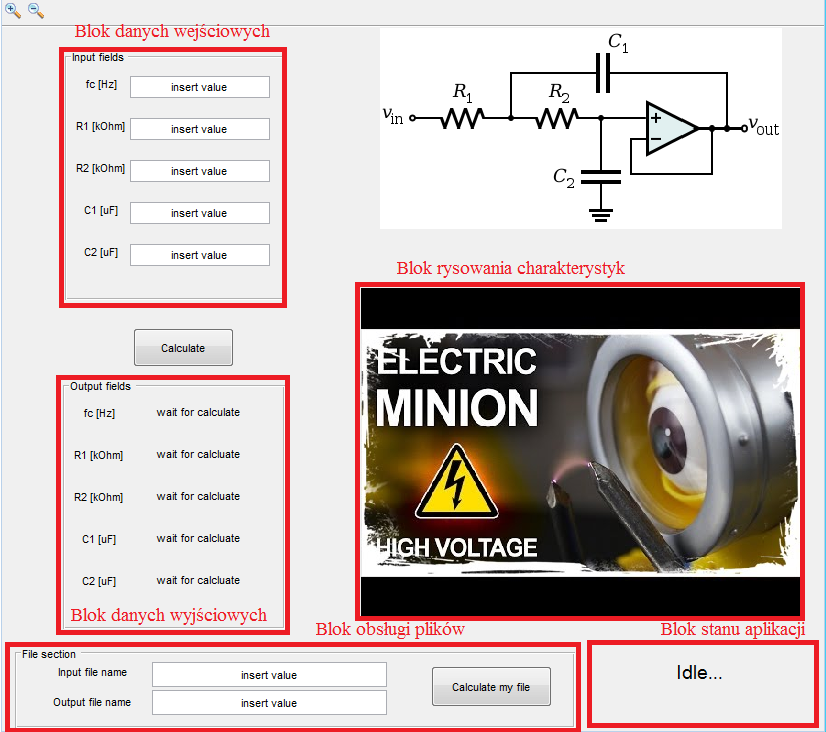
\includegraphics[width=\textwidth]{../Pictures/i1.png}
 					 \caption{Podział okna programu na bloki główne.}
					 \label{fig:bloki}
			\end{figure}

	\subsection{Wprowadzanie danych przez użytkownika}
		Aby policzyć wartości elementów pasywnych (opór rezystora i pojemność kondensatora)
		dla pojedynczego układu należy:
		\begin{enumerate}
			\item Wprowadzić w pole fc bloku danych wejściowych wartość oczekiwanej
			częstotliwości granicznej filtru wyrażoną w Hz.
			\item Wprowadzić w pole R1 albo R2 bloku danych wejściowych wartość rezystancji
			wybranego rezystora wyrażoną w k$\Omega$ . W przypadku wprowadzenia wartości 
			dla jednego z rezystorów pole odpowiadające drugiemu rezystorowi staje się
		 	nieaktywne, aby odblokować to pole należy usunąć wartość z uzupełnionego pola.
		 	\item Wprowadzić w pole C1 albo C2 bloku danych wejściowych wartość pojemności
			wybranego kondensatora wyrażoną w uF. W przypadku wprowadzenia wartości 
			dla jednego z kondensatorów pole odpowiadające drugiemu kondensatorowi staje się
		 	nieaktywne, aby odblokować to pole należy usunąć wartość z uzupełnionego pola.
		 	\item Kliknąć przycisk "Calculate" rozpoczynający proces obliczeniowy, po 
		 	zakończeniu którego wartości wszystkich elementów pasywnych układu zostają
		 	wyświetlone w bloku danych wyjściowych, a w bloku rysowania charakterystyk
		 	wyświetlone zostają charakterystyki amplitudowo-fazowe dla danego układu.
		\end{enumerate}		

		Na rysunku nr. \ref{fig:dane} przedstawiony został widok aplikacji po 
		wykonaniu obliczeń dla danych wprowadzonych przez użytkownika.

		\pagebreak				
				
		\begin{figure}[!htbp]
 				\centering
					 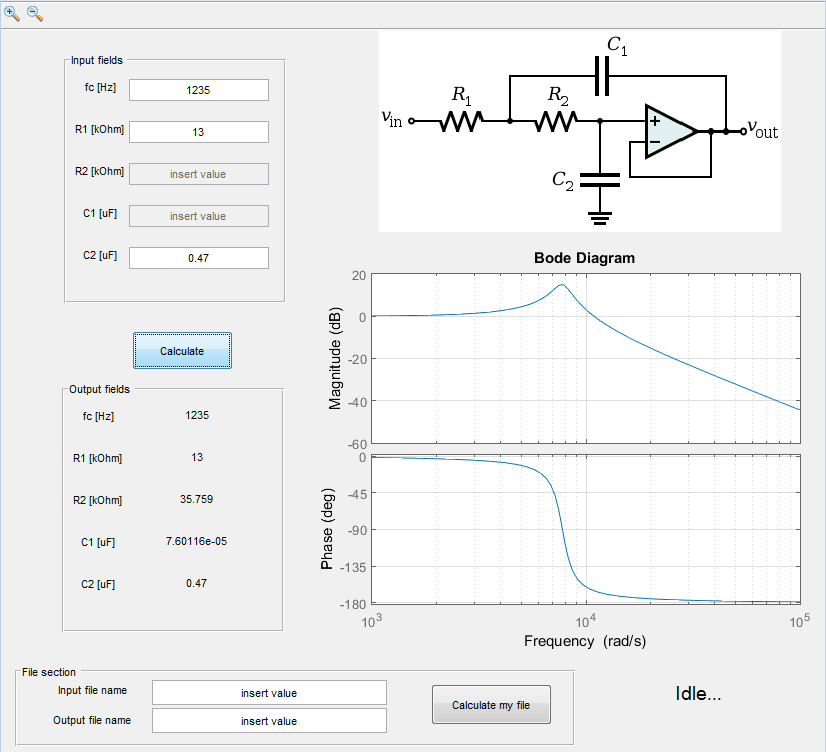
\includegraphics[width=\textwidth]{../Pictures/i2.png}
 					 \caption{Widok okna po zakończeniu obliczeń na podstawie danych 
 					 wprowadzonych przez użytkownika.}
					 \label{fig:dane}
			\end{figure}
			

	\subsection{Wprowadzanie danych z pliku}
	
		Aby policzyć wartości elementów pasywnych dla większej ilości układów
		do programu można wprowadzić plik w formacie .xls gdzie pojedynczy układ jest 
		reprezentowany przez pojedynczy wiersz zgodnie z opisem w rozdziale nr.
		\ref{sec:format}. Aby tego dokonać należy:
		
		\begin{enumerate}
			\item Przygotować plik z danymi wejściowymi zgodnie z opisanym formatem
			danych i umieścić go w katalogu uruchomieniowym aplikacji.
			\item Wprowadzić nazwę pliku z danymi wejściowymi
			w pole "Input file name" w oknie aplikacji.
			\item Wprowadzić nazwę pliku do którego zapisane zostaną dane wyjściowe 
			w pole "Otput file name" w oknie aplikacji.
			\item Kliknąć przycisk "Calculate my file" rozpoczynający proces wczytania 
			danych, dokonania obliczeń i zapisania wyników do pliku.
		\end{enumerate}
			
\section{Format danych}
	\label{sec:format}

	Dane wejściowe programu są liczbami dodatnimi opisującymi filtr:
	\begin{itemize}
				\item fc - częstotliwość graniczna filtru
				\item r1 - wartość rezystancji opornika R1 [kOhm]
				\item r2 - wartość rezystancji opornika R2 [kOhm]
				\item c1 - wartość pojemności kondensatora C1 [uF]
				\item c2 - wartość pojemności kondensatora C2 [uF]
	\end{itemize}
	
	podczas wprowadzania danych należy pamiętać, że należy podać wartości 
	fc, oraz po jednej ze zbiorów \{r1, r2\}, \{c1, c2\}. Program posiada zabezpieczenia
	przez niepoprawnym wprowadzeniu danych.  \\
	W przypadku wprowadzania danych z pliku .xls należy utworzyć 5 kolumn, które 
	reprezentują wartości opisujące filtr w kolejności wyżej wymienionej.
	Wartości elementów do obliczenia muszą w pliku wynosić 0.
	Każdy kolejny wiersz traktowany jest jako kolejny układ do obliczenia.
	Plik z danymi wyjściowymi reprezentowany jest podobnie jak plik wejściowy
	 w pięciu kolumnach
	 z tą różnicą, że występuje wiersz nagłówkowy opisujący kolumny.
	 Wiersze niespełniające powyższych kryteriów będę przez program ignorowane.
	 Jeżeli w pliku wystąpi więcej niż 5 kolumn cały plik zostanie zignorowany.
	 Poprawny format danych wejściowych i wyjściowych w plikach został przedstawiony
	 na rysunku nr. \ref{fig:plik}.
	 
	 		\begin{figure}[!htbp]
 				\centering
					 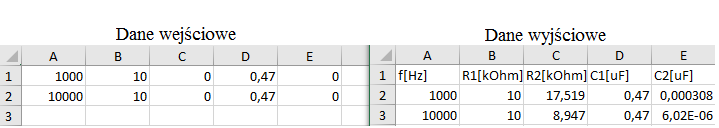
\includegraphics[width=\textwidth]{../Pictures/plik.png}
 					 \caption{Format danych w pliku wejściowym i wyjściowym.}
					 \label{fig:plik}
			\end{figure}

\section{Możliwy rozwój projektu}

	\begin{enumerate}
		\item Dodanie opcji generowania charakterystyk Bodego dla wprowadzonych przez 
		użytkownika kompletnych danych opisujących filtr.
		\item Wprowadzenie algorytmu doboru elementów pasywnych filtru spośród wartości 
		należących do istniejących szeregów np. E24.
	\end{enumerate}

\end{document}

